\documentclass[conference]{IEEEtran}

\usepackage[
backend=biber,
style=numeric,
sorting=none
]{biblatex}
\addbibresource{bibliography.bib}

\usepackage{amsmath}
\usepackage{algorithmic}
\usepackage{booktabs}
\usepackage{comment}

\usepackage{pgfplots}
\usepackage{pgfplotstable}
\pgfplotsset{compat=1.17}

\usepackage{xcolor}
\definecolor{redbullet}{RGB}{234,67,53}
\definecolor{bluebullet}{RGB}{66,133,244}
\definecolor{yellowbullet}{RGB}{251,188,4}
\definecolor{greenbullet}{RGB}{52,168,83}

\def\BibTeX{{\rm B\kern-.05em{\sc i\kern-.025em b}\kern-.08em
    T\kern-.1667em\lower.7ex\hbox{E}\kern-.125emX}}

% correct bad hyphenation here
\hyphenation{op-tical net-works semi-conduc-tor}

\begin{document}

\title{Application of Correlation Coefficients to Measurements of Decentralization}

\author{
  \IEEEauthorblockN{Simon Brown}
  \IEEEauthorblockA{\textit{ConsenSys Software Inc.}\\
  simon.brown@consensys.net}
  \and
  \IEEEauthorblockN{Leonardo Bautista-Gomez}
  \IEEEauthorblockA{\textit{Miga Labs}\\
  leobago@protonmail.com}
}

% make the title area
\maketitle

\begin{abstract}
There have been several studies into measuring the level of decentralization in Ethereum through applying various indices to indicate relative dominance of entities in different domains in the ecosystem.  However, these indices do not capture any correlation between those different entities, that could potentially make them the subject of external coercion, or covert collusion.  We propose an adapted index that adjusts the relative dominance of entities based on the application of correlation factors.  We posit that this approach produces a more nuanced and accurate index of decentralization.
\end{abstract}

% Note that keywords are not normally used for peerreview papers.
\begin{IEEEkeywords}
blockchain, Ethereum, decentralization, cryptocurrency, cryptoeconomics
\end{IEEEkeywords}

\section{Introduction}

There have been several attempts to model a heuristic to measure the level of decentralization in the Ethereum ecosystem, that have relied on various techniques and indices that have been borrowed from the fields of economics and ecology \cite{wu2020coefficient} \cite{gupta2018gini} \cite{gochhayat2020measuring} \cite{lee2021dq}.  These include indices such as the Gini index and the Herfindahl–Hirschman Index, as well as several indices that are derived from the measurement of entropy \cite{brown2023measuring}.  When used in combination, these measurements reveal useful insights into the relative market share and/or share of resources of various entities, which can indicate the areas of concentration or diffusion of control and influence in the ecosystem.

While these measurements can prove useful in measuring decentralization at a high level, they fail to capture the nuance in the correlation between various entities within the ecosystem, which can lead to subtle implicit collusion and/or potential coercion by external actors.  We therefore propose a model that seeks to capture the level of correlation between entities in the ecosystem across a number of dimensions, and present our findings from applying the model to available network data.  We demonstrate how the level of correlation between independent entities can reduce the effective level of decentralization in certain cases, while increasing the effective level of decentralization other cases.

This paper is organized as follows: in section II we discuss the background and motivation for this research, in section III we describe our methodology, and the various calculations used in our model.  In section IV we outline the results of applying our model to the underlying dataset.  We summarize the results and learnings in section V, and finally discuss future work and areas for further research in section VI.

\section{Background}

Ethereum currently has over 916,000 validators \cite{beaconchain2024} attached to approximately 5,000 to 6,000 nodes [CITE - Miga Labs], out of a total of approximately 14,000 nodes across the entire network \cite{nodewatch2024}.

Many validator clients are controlled by staking pools, with only about 25\% of the validator set being independent solo stakers \cite{dune2024}.  Several staking pools have garnered a relatively large market share, some who employ a number of different node operators to run nodes on the network, to which validators are attached.  Node operators can attached any number of validators to the nodes they run, and can employ any combination of execution client and consensus client, of which there are approximately 6 widely adopted clients of each available.

Furthermore, node operators may choose to connect to independent, third-party block builders to source the blocks that the validators attached to their nodes propose to the network. Nodes connect to builders via relayers in the mev-boost system.  Relayers are run by other independent providers and provide a quasi-escrow service for block builders and validators to negotiate payment and delivery for blocks.

\section{Motivation}

At a high level, we can observe patterns within the ecosystem that highlight potential areas of concern, including potential implications for the network's security in terms of client diversity \cite{clientdiversity2024}, or an over-reliance on certain infrastructure providers (e.g. cloud providers, relayers etc.), as well as the network's ability to withstand coercion from regulatory overreach in any number of jurisdictions \cite{wahrstatter2023}. These insights do not necessarily reveal any indication of why these patterns of concern occur in the first place however.

An example of why the correlation between entities is important to measure is when considering the market share of staking pools. Different staking pools have different policies regarding node operators, including geographical location, and client diversity \cite{vanom2024}.  Through segmenting the validator set by staking pool, we can measure the level of decentralization within each staking pool, by measuring the diversity of node operators, clients and relays within each staking pool, adjusted for correlation to each other. The resulting measurement can then be used to adjust the market share of staking pools to more accurately reflect the effective level of decentralization.  Similarly, while the market concentration of node operators is ostensibly diffuse, through measuring the correlation between node operators across several dimensions, we can start to see that a more accurate level of concentration than simply looking at the market share alone.

\section{Data Sources}

Our study analyses two discrete datasets from two independent sources:

\begin{itemize}
    \item Dataset A: sourced from rated.network, which pertains to node operators and staking pools, sourced on the 15th January 2024, and contains data from the preceding 30 days.
    \item Dataset B: sourced from Miga Labs, and which contains data pertaining to individual consensus nodes on the network.  This dataset includes the number of attestation subnets each node advertises, but only includes nodes that advertise more than 2 subnets.
    \item Dataset C: sourced from Miga Labs, and which contains data pertaining to individual consensus nodes on the network, but with a smaller sample size, less than 500 records.  This dataset contains the specific number of validators nodes attached to each node.
\end{itemize}

Each dataset contains a discrete set of attributes, which we analyze for patterns of correlation.  The attributes that are analyzed in each dataset include:

\begin{itemize}
    \item \textbf{Dataset A} (Node Operators):
    \begin{itemize}
        \item Market share of node operator
        \item Percentage breakdown staking pools served
        \item Percentage breakdown of client software
        \item Percentage breakdown of relayers used
    \end{itemize}
    \item \textbf{Dataset B} (Individual Nodes):
            \begin{itemize}
                \item Country of Operation
                \item Client Software
                \item ISP / Datacenter
                \item Number of advertised attestation subnets
            \end{itemize}
    item \textbf{Dataset C} (Individual Nodes):
            \begin{itemize}
                \item Country of Operation
                \item Client Software
                \item ISP / Datacenter
                \item Number of validator clients
            \end{itemize}
\end{itemize}

\section{Methodology}

Our analysis applies several calculations to each dataset in order to attempt to identify any correlations between entities in the dataset across various attributes, and any correlations between specific attributes.

We adapt the standard Herfindahl–Hirschman Index to account for potential correlations between staking pools, and we apply the same analysis to node operators.

We examine the level of correlation between variability in attributes in dataset A, in order to identify any correlation between a staking pool and the level of client diversity, or the range of node operators or relayers that are used by that staking pool.

We attempt to calculate a correlation between the market share of node operators and the consensus clients they run, and relayers that they use, by mapping each percentile of market share to the total number of clients / relays used by staking pools and node operators in that percentile.

Our analysis also examines individual nodes on the network by calculating any correlation between individual nodes in dataset B using standard statistical measurements of correlation.  We also employ a novel approach for finding correlation between attributes.

\subsection{Standard Herfindahl–Hirschman Index}

Our model uses the Herfindahl–Hirschman Index as a basis for measuring the market concentration of staking pools and node operators.  The Herfindahl–Hirschman Index is a widely adopted economic index for measuring market concentration across a number of economic sectors \cite{OECD2021}.

The HHI relies on market percentage shares, and is defined as the sum of the square of the percentage share of each entity in a population.  It therefore results in a value close to 0 for a population in which each entity has a relatively equal share, but approaches $100^2$ in a population which is dominated by a relatively small number of entities.

\begin{comment}
It is defined according to the following formula, where $s$ is the percentage market share of each entity $i$.

\[
HHI = \sum_{i} s_i^2
\]
\end{comment}

\subsection{Modified Herfindahl–Hirschman Index}
This is calculated by summing the market share of every entity multiplied by the market share of every other entity and an additional correlation factor, that indicates how correlated the respective entities are.  The correlation factor, $\rho_{ij}$, between entities $i$ and $j$, adjusts their respective market shares to account for their level of similarity across various attributes.

\[
HHI' = \sum_i \sum_j \left(s_i \cdot s_j \cdot \rho_{ij}\right) \times 100
\]

Where $s_i$ and $s_j$ represent the market shares of entities $i$ and $j$, respectively. When applied to the set of staking pools derived from dataset A, each entity is an unique staking pool, and the correlation factor $\rho_{ij}$ is then calculated for each pairwise comparison in the dataset as follows:

Let $R_i$, $C_i$ and $O_i$ be the sets of relays, clients, and operators for entity $i$, respectively. Similarly, let $R_j$, $C_j$ and $O_j$ be the sets of relays, clients, and operators for entity $j$.  The values in each set represent the percentage of each relay, client, or operator employed by the respective entity, and therefore the sum total of all values in a set is 100.

The correlation factor $\rho_{ij}$ between entities $i$ and $j$ is defined as the sum of the minimum of each corresponding value in the sets $R_i$, $C_i$ and $O_i$ and the sets $R_j$, $C_j$ and $O_j$. This can be expressed as follows:

\[
\sum_{k=1}^{|R|} \min(R_{ik}, R_{jk}) + \sum_{k=1}^{|C|} \min(C_{ik}, C_{jk}) + \sum_{k=1}^{|O|} \min(O_{ik}, O_{jk})
\]

In other words, the correlation factor is derived from examining the clients, relays and operators that each pair of staking pools have in common, and taking the minimum percentage that each staking pools uses in each case, and adding those percentages together.

Each correlation factor that is calculated is only considered when it's value is greater than a baseline $\beta$, where the baseline is the total number of staking pools divided by the number of clients, relays, node operators respectively.  Without loss generality, consider a set of pools $P$, that all run a combination of some client software $C$.  In the case of perfect uniform distribution of client software usage, each pool would have a baseline correlation factor of $\beta = \frac{|P|}{|C|}$.  We therefore only consider $C_{ij}$ when $C_{ij} > \beta$.

We calculate and compare both the standard HHI and and the modified HHI for both staking pools and node operators.  In the case of node operators, the correlation factor only considers clients and relayers.

\subsection{Calculating correlation between variability in attributes}

Our analysis attempts to measure any correlation between the level of variability in clients, relayers and node operators across staking pools. This is done to try to identify if there is a correlation between the size of a staking pool and the level of client diversity, or the range of node operators or relayers that are used.

This is done by first calculating the coefficient of variance in the percentages of relayers, clients and node operators used by each staking pool. From this we obtain a matrix with a row for each staking pool, a column for market share, and columns for the coefficients of variation for clients, relayers and node operators.  We then calculate the $R^2$ value for each pairwise combination of columns to identify any potential correlation.

The coefficient of variation (CV) as a measure of relative variability is calculated as the ratio of the standard deviation ($\sigma$) to the mean ($\mu$) of a set of clients, relayers and node operators respectively, defined as:

\[ CV = \left( \frac{\sigma}{\mu} \right) \times 100 \]

Using the resulting matrix of staking pools and the coefficient of variation of their attributes: clients, relayers and node operators, we can then calculate the Pearson correlation coefficient \cite{pearson1895} for each pairwise combination of attributes.  The Pearson correlation coefficient, $r$, is well know to any student of statistics and is defined as:

\[
r = \frac{\sum{(X_i - \bar{X})(Y_i - \bar{Y})}}{\sqrt{\sum{(X_i - \bar{X})^2}\sum{(Y_i - \bar{Y})^2}}}
\]

\vspace{3pt}

Where $X_i$ and $Y_i$ are the individual data points of attributes $X$ and $Y$ and $\bar{X}$ and $\bar{Y}$ are the means of attributes $X$ and $Y$, respectively.  For each $r$ value, we square the result to obtain the coefficient of determination, $R^2$, which indicates any potential correlation between attributes.

We also apply the above analysis to node operators, whereby we attempt to analyze whether there is any correlation between variability in the market share of the node operators and the clients that they run or relayers they use.

\subsection{Correlation between operators size, clients and relayers}

Our analysis also attempts to calculate a correlation between the market share of node operators and the consensus clients they run.

This  involves analyzing the set of node operators $K$, each possessing a market share represented by $m$, along with the percentage breakdown of the clients they run, denoted as $c = { c_1, c_2 . . . c_n }$. Each $c_i$ signifies the percentage of a specific client in the known client set $C$, run by the operator $k_i$ in $K$.

A function is employed to construct a matrix, denoted as $M$, wherein each row corresponds to a market share percentile $d \in \left\{0, 1, ... 9\right\}$, and each column corresponds to a client $c \in C$. In this matrix, each column aggregates the sum of percentages of that client that is run by all node operators in the dataset possessing the respective market share percentile.

To generate this matrix, the function $f: m_i \mapsto d$, iterates through the set $K$. For each entity $k_i \in K$, it maps the entity's percentage market share $m_i$ to the corresponding percentile $d \in \left\{0, 1, ... 9\right\}$ and increases the values in the columns of $M$ corresponding to each client $c_j \in C$ by the percentage run by node operator $k_i$.

The resulting matrix provides view of any correlation of market share of node operators to the clients they use, and the diversity of clients they use, visualized as:

\[
M = \begin{bmatrix}
m_1 & M_1^1 & M_1^2 & \ldots & M_1^{\nu} \\
m_2 & M_2^1 & M_2^2 & \ldots & M_2^{\nu} \\
\vdots & \vdots & \vdots & \ddots & \vdots \\
m_n & M_{\eta}^0 & M_{\eta}^1 & \ldots & M_{\eta}^{\nu}
\end{bmatrix}
\]

where $\nu$ is the size of the set of clients, and $\eta$ is the size of the set of node operators.

This analysis can indicate if any particular client is favoured by larger or smaller node operators. The process is repeated for relayers as well, whereby we try to establish any correlation between the market share of node operators and which relayers they use, as well as the number of relayers they use.

\subsection{Calculating correlation between individual nodes}

In order to determine if there is any correlation between individuals nodes on the network across various attributes, we analysed the dataset from Miga Labs, which contain data on individual nodes on the network, including country, client, ISP, number of attestation subnets advertised. For the purposes of our study, we limited our analysis to nodes that had greater than 2 attestation subnets advertised, as these are the most likely to be nodes with validator clients attached.

\subsubsection{Calculating Chi-squared value between attributes}

We analyzed the data by calculating the Chi-squared value between each pairwise attribute, we then then calculated the corresponding p-value, and finally derived the Cramers-V value.

To do this we first generate a contingency table for each pairwise comparison of attributes in the dataset.  Each contingency table has rows for each value of attribute A, and columns for each value of attribute B, where each cell contains the frequency of occurrences for each combination of values of attribute A and B respectively. The Chi-squared value is then calculated as:

\[
\chi^2 = \sum \frac{(O_{ij} - E_{ij})^2}{E_{ij}}
\]

Where $O_{ij}$ is the observed frequency in cell $(i, j)$, and $E_{ij}$ is the expected frequency in cell $(i, j)$, calculated as:

\[
E_{ij} = \frac{(\text{row sum})(\text{column sum})}{\text{total number of nodes}}
\]

\subsubsection{Calculating Cramers-V value between attributes}

We also calculate the Cramers-V value \cite{akoglu2018user} for each pairwise as a complimentary measurement to the result of both the Chi-squared value and p-value of each pairwise comparison of attributes.  While taking a single measurement in isolation can give us unreliable results, a combination of measurements can give us more confidence in the results where they broadly align.

Cramer's V is calculated using the following formula:

\[ V = \sqrt{\frac{\chi^2}{n \cdot \min(k-1, r-1)}} \]

Where:
\begin{itemize}
    \item $\chi^2$ is the chi-squared statistic obtained from the contingency table, as previously calculated,
    \item $n$ is the total number of observations in the table,
    \item $k$ is the number of columns in the table,
    \item $r$ is the number of rows in the table.
\end{itemize}

\vspace{8pt}

Cramer's V ranges from 0 to 1, where 0 indicates no correlation between the attributes, and 1 indicates they are totally correlated with one another.  While this allows us to determine if there is any correlation between the market share of node operators and the consensus clients they run, we also apply this analysis to size of node operators and relayers they use.

\subsection{Ranking the level of correlation between attributes}

Our analysis also includes a function to determine which attributes display the highest amount of correlation between individual nodes in the network.

For every record in the dataset, we compare it to every other record in the dataset along a specific attribute, including country, client, ISP, and number of attestation subnets advertised.

Where the attributes are equal for each record, we record a 1, where they are not equal, we record 0.
The result is a bitstring for each attribute from which we can derive a hamming weight.
The process can be described as incrementing a count every time the attribute for each record being compared is equal, and is essentially a method for deriving a count for each unique value observed in a specific attribute. We then repeat the entire process for the next attribute.

The result is a series of hamming weights for each record compared to every other record, for each attribute. We then add all the hamming weights together for each record, so every record has an aggregate hamming weight, resulting in a table with the record index in column 1, a column for the hamming weight of each attribute, and a column for the sum of all hamming weights for that record.

This aggregate hamming weight indicates the level of correlation of the respective node to other nodes, and allows us to rank the dataset to help identifying patterns between correlations. The hamming weights in each column represent the sum of all observances of the value of the attribute of the respective record.

The process is defined formally as:

Let \( N \) be the number of records in the dataset, and \( M \) be the number of attributes.  For each pair of records \( i \) and \( j \) (\( i, j \in \{1, 2, \ldots, N\} \) and \( i \neq j \)), and for each attribute \( k \) (\( k \in \{1, 2, \ldots, M\} \)), we define a binary function \( \delta \left( i_k,j_k \right) \) using the Kronecker delta function:

\[
\delta \left( i_k,j_k \right) = \begin{cases} 1 & \text{if } i_k = i_k \\ 0 & \text{if } i_k \neq j_k \end{cases}
\]

The Hamming weight \( H_{ik} \) for record \( i \) and attribute \( k \) is the sum of all binary values for that attribute across all pairwise comparisons:

\[ H_{ik} = \sum_{j=1, j\neq i}^{N} \delta \left( i_k,j_k \right) \]

The aggregate Hamming weight \( A_{i} \) for record \( i \) is the sum of Hamming weights across all attributes:

\[ A_{i} = \sum_{k=1}^{M} H_{ik} \]

The final table can be represented as a matrix \( T \) with \( N \) rows and \( M+2 \) columns, where the first column contains the record index, columns \( 2 \) to \( M+1 \) contain the Hamming weights for each attribute, and the last column contains the aggregate Hamming weight:

\[ T = \begin{bmatrix} 
1 & H_{1,1} & H_{1,2} & \ldots & H_{1,M} & A_{1} \\
2 & H_{2,1} & H_{2,2} & \ldots & H_{2,M} & A_{2} \\
\vdots & \vdots & \vdots & \vdots & \vdots & \vdots \\
N & H_{N,1} & H_{N,2} & \ldots & H_{N,M} & A_{N}
\end{bmatrix} \]

\vspace{2pt}

This matrix \( T \) represents a table with the record index, individual Hamming weights for each attribute, and the aggregate Hamming weight for each record.

\section{Results}

We presents the results from the application of each calculation described in the previous section to the dataset A and B.  The results are detailed in the relevant subsections that follow.  Discussion of the results and their possible interpretations, as well as any future work that the results suggest, is expanded upon in the conclusion section.

\subsection{Calculating correlation between variability in attributes}

Our analysis first examines the level of variability in the clients and relayers used by each node operator.  Each node operator is given a coefficient of variance for each attribute, calculated from the respective percentages of clients and relayers that the node operator uses. We then attempt to calculate any correlation between the variability in each attribute by calculating the $R^2$ value for each pair of attributes.  This method is also applied to the variability in clients, relayers and node operators that each staking pool uses.

\subsubsection{Correlation of variability across attributes for Node Operators}

The following table presents the $R^2$ values for comparison of variability between attributes in datasets A with respect to node operators. As can be seen from the results below, there is strong correlation between the market share of the node operator and the variability in the distribution of relays they have procured blocks from. This is likely explained by the observation that larger node operators tend to connect to more relayers then smaller operators and solo stakers, who tend to connect to only one or a small set of relayers.  However, this observation may be partially explained by the fact solo stakers propose blocks relatively infrequently, and may have proposed only one or two blocks within the sample period, and this may be represented in the data in terms of which relayers they won those blocks from.  In this context they may have connected to multiple relayers, but only proposed blocks that were sourced from one or two relayers.

\begin{table}[htbp]
    \centering
    \normalsize
    \begin{tabular}{p{3.9cm}r}
        \toprule
        Pairwise Comparison & Strength of Correlation ($R^2$) \\
        \midrule
        Market Share vs. Clients & 0.16 \\
        Market Share vs. Relayers & 0.37 \\
        Relays vs. Clients & 0.16 \\
        \bottomrule
    \end{tabular}
\end{table}

\subsubsection{Correlation of variability across attributes for Staking Pools}

The table \ref{tab:r2-value-staking-pools} presents the $R^2$ values for comparison of variability between attributes in datasets A with respect to staking pools.

\begin{table}[htbp]
    \centering
    \normalsize
    \renewcommand{\arraystretch}{1.2}
    \begin{tabular}{|p{6cm}|c|}
        \hline
        \textbf{Relationship} & \textbf{$R^2$ Value} \\
        \hline
        Market Share vs. Clients & 0.01 \\ \hline
        Market Share vs. Relays & 0.02 \\ \hline
        Market Share vs. Operators & 0.0 \\ \hline
        Relays vs. Clients & 0.36 \\ \hline
        Relays vs. Node Operators & 0.11 \\ \hline
        Clients vs. Node Operators & 0.07 \\ \hline
    \end{tabular}
    \vspace{10pt}
    \caption{$R^2$ Values for Different Relationships}
    \label{tab:r2-value-staking-pools}
\end{table}

As can be seen from table \ref{tab:r2-value-staking-pools}, the only value of any significance is the $R^2$ value for Relays vs Clients.  This indicates a strong correlation between the variability in consensus clients that are used by a staking pool, and the variability in the relays that they are using.  This would suggest that staking pools that employ node operators with a higher level client of diversity also connect to multiple relayers.  While it is not surprising that staking pools with a larger market share may have multiple node operators, the results do not show a high correlation between market share and clients or relays, \textbf{indicating that the size of the staking pool does not necessarily correlate with their policies around client diversity or relayer diversity.}

\subsection{Calculating Standard and Modified Herfindahl–Hirschman Indices}

\subsubsection{Herfindahl–Hirschman Indices for Node Operators}

In observing the difference between the standard HHI index and the modified HHI index for node operators, we see a significant difference.  The \textbf{standard HHI yields a value of 66}, indicating a highly unconcentrated market of node operators.  This would suggest a very healthy level of diffusion within the node operator set, and is representative of a dataset of 2,496 records with only 22 operators that have a market share of above 1\%, and only 4 that have a market share between 2\% and 4\%.  The modified HHI yields a value of 1,223 without baseline compensation, but yields a value of 0 when baselined, which reinforces the conclusion that there is no significant level of overt correlation between node operators.

This value more accurately represents the fact that most relayers are using the same clients and relayers.  Given that there are only 6 consensus clients and 5 relayers with any significant market share, it is not surprising that we see this result in a population of 2,496 node operators.

\subsubsection{Herfindahl–Hirschman Indices for Staking Pools}

In observing the difference between the standard HHI index and the modified HHI index for node operators, we see a notable difference.  The standard HHI for staking pools yields a value of \textbf{1,135}, indicating a low-to-moderate level of market concentration in terms the standard interpretation of the HHI \cite{usdoj2015}.  The modified HHI yields a value of \textbf{3,183}, almost 3 times greater than the standard HHI.  Our analysis identified 13 unique staking pools, using 6 clients and 6 relayers in numerous combinations.

It is worth noting however, that a direct comparison between the standard HHI and modified HHI can be misguiding.  The modified HHI should be based against some benchmark that is established over time, or a defined heuristic baseline.

\subsection{Analysis of Individual Nodes}

\subsubsection{Measuring the correlation between attributes in Dataset B}

We present the results of analysing the correlation between individual nodes on the network in dataset B. The results are shown in table \ref{tab:pairwise-comparisons-dataset-b}, for the Chi-squared, p-value and Cramér's V value each each pairwise comparison of attributes.

\begin{table}[ht]
    \centering
    \renewcommand{\arraystretch}{1.5}
    \begin{tabular}{|p{2.5cm}|c|c|c|}
        \hline
        \textbf{Comparison} & \textbf{Chi-squared} & \textbf{P-value} & \textbf{Cramér's V} \\
        \hline
        Country v Client & 866.56 & \textless 0.01 & 0.22 \\ \hline
        Country v ISP & 83,766.05 & 0 & 0.82 \\ \hline
        Country v Subnets & 4,625.32 & \textless 0.01 & 0.12 \\ \hline
        Client v ISP & 2,409.07 & \textless 0.01 & 0.21 \\ \hline
        Client v Subnets & 969.73 & \textless 0.01 & 0.23 \\ \hline
        ISP v Subnets & 30,525.86 & 0 & 0.31 \\ \hline
    \end{tabular}
    \vspace{10pt}
    \caption{Pairwise Comparisons with Chi-squared Test Statistics}
    \label{tab:pairwise-comparisons-dataset-b}
\end{table}

\begin{comment}
The values above are transcribed to be in more readable format below.  The strength of association is based on the Chi-Squared value.

\begin{table}[htbp]
    \centering
    \normalsize
    \begin{tabular}{p{4cm}p{4cm}}
        \toprule
        Pairwise Comparison & Strength of Association \\
        \midrule
        Country / Subnets & Small \\
        Country / Client & Small-to-Medium \\
        Client / ISP & Small-to-Medium \\
        Client / Subnets & Small-to-Medium \\
        ISP / Subnets & Moderate \\
        Country / ISP & Strong \\
        \bottomrule
    \end{tabular}
\end{table}
\end{comment}

As is expected, there is a strong correlation between the country of operation and the ISP used.  This is exactly what we would expect to see given that most ISPs only serve their domestic market.

There is also a moderate level of correlation between the ISP used and the number of attestation subnets advertised.  As ISPs in this context also include public cloud providers, this correlation may suggest that nodes advertising multiple attestation subnets, i.e. nodes that likely have multiple validators attached, are often using the same public cloud provider, e.g. AWS, Azure etc.

\begin{figure}[htbp]
    \centering
    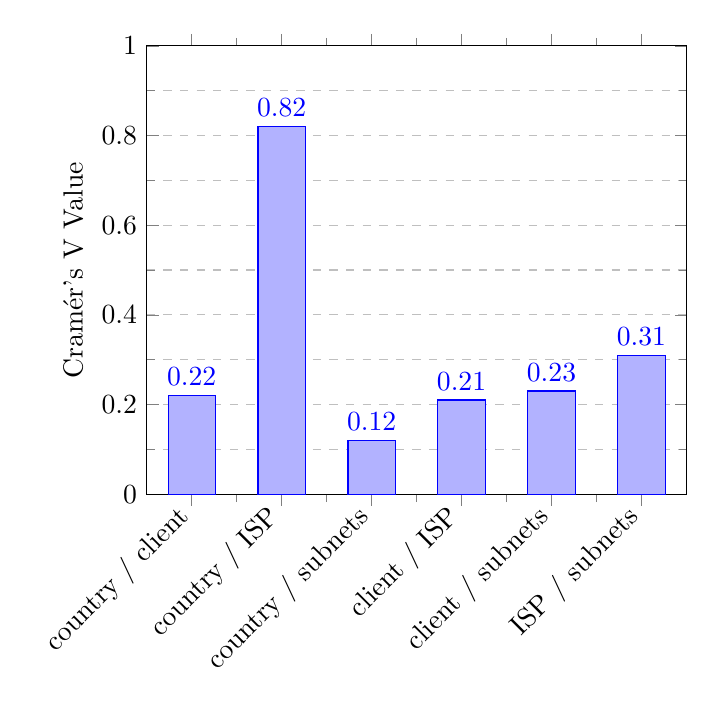
\begin{tikzpicture}
      \begin{axis}[
          ybar,
          bar width=0.6cm,
          ylabel={Cramér's V Value},
          xtick=data,
          xticklabels={
              country / client,
              country / ISP,
              country / subnets,
              client / ISP,
              client / subnets,
              ISP / subnets
          },
          ymajorgrids=true,
          yminorgrids=true,
          grid style=dashed,
          minor x tick num=1,
          minor y tick num=1,
          x tick label style={rotate=45, anchor=east, align=right},
          ymin=0, ymax=1,
          legend pos=north west,
          legend style={font=\footnotesize},
          nodes near coords,
          nodes near coords align={vertical},
          ]
        
          \addplot coordinates {(1, 0.22) (2, 0.82) (3, 0.12) (4, 0.21) (5, 0.23) (6, 0.31)};
        
      \end{axis}
    \end{tikzpicture}
    \caption{Relative level of correlation between attributes}
    \label{fig:relative-level-of-correlation-between-attributes}
\end{figure}

An interesting observation from the results shown in figure \ref{fig:relative-level-of-correlation-between-attributes} is that there is a relatively low correlation between the country that nodes are based in and the number of attestation subnets that they advertise.  It is widely acknowledged that there is  strong concentration of nodes in the US and EU geographical regions, this low correlation would indicate that nodes that have multiple validators attached to them, and therefore likely to be operated by node operators serving staking pools, may be more geographically distributed.  This hypotheses will require further research however.

We also include the results of the same calculations applied to dataset C, which are included in table \ref{tab:pairwise-comparisons-dataset-c}.  This analysis includes measures of correlation between the number of validators attached to clients and other attributes, including country, ISP and clients.

\begin{table}[ht]
    \centering
    \renewcommand{\arraystretch}{1.5}
    \begin{tabular}{|p{2.5cm}|c|c|c|}
        \hline
        \textbf{Comparison} & \textbf{Chi-squared} & \textbf{P-value} & \textbf{Cramér's V} \\
        \hline
        Validators v Client & 460.7 & \textless 0.01 & 0.25 \\ \hline
        Validators v Country & 3,508.91.56 & \textless 0.01 & 0.28 \\ \hline
        Validators v ISP & 14,542.56 & \textless 0.01 & 0.38 \\ \hline
        Client v Country & 283.82 & \textless 0.01 & 0.2 \\ \hline
        Client v ISP & 1,260.46 & \textless 0.01 & 0.4 \\ \hline
        Country v ISP & 16,500.88 & 0 & 0.79 \\ \hline
    \end{tabular}
    \vspace{10pt}
    \caption{Pairwise Comparisons with Chi-squared Test Statistics}
    \label{tab:pairwise-comparisons-dataset-c}
\end{table}

We observe a similar trend in the analysis of dataset C, whereby the there is strong correlation between a node's country of operation and the ISP.  We also observe moderately strong correlation between the client software and the ISP, as well as the number of validators and the ISP.

\subsection{Correlation between node operator market share and clients and relayers}

\subsubsection{Operator market share and clients used}

The scatter plot in figure \ref{fig:average_client_percentage_by_percentile} show the correlation between the market share of node operators in Dataset A, and the average percentage of each client that node operators in the respective market share percentile use.

\begin{figure}[htbp]
  \centering
  \begin{tikzpicture}
    \begin{axis}[
      only marks,
      xlabel={Percentile of Network Penetration},
      ylabel={Percentage Client Use},
      symbolic x coords={0, 1, 2, 3},
      xtick=data,
      xmajorgrids=true,
      ymajorgrids=true,
      grid style=dashed,
      xminorgrids=true,
      yminorgrids=true,
      minor x tick num=1,
      minor y tick num=1,
      legend style={at={(0.5,-0.225)},anchor=north,font=\footnotesize,draw=gray!50,
                    legend columns=3,
                    /tikz/every even column/.append style={column sep=0.5cm},
                    /tikz/every odd column/.append style={column sep=0.5cm}},
      legend entries={Nimbus,Prysm,Lighthouse,Teku,Lodestar,Unknown},
    ]

    \pgfplotstableread[col sep=comma]{data/average_client_percentage_by_percentile.csv}\datatable

    \foreach \col in {1,...,6} {
      \pgfplotstablegetcolumnnamebyindex{\col}\of\datatable\to\colname
      \addplot table[x=Network Penetration, y index=\col] {\datatable};
    }

    \end{axis}
  \end{tikzpicture}
  \caption{Average Client Percentage by Node Operator Market Share}
  \label{fig:average_client_percentage_by_percentile}
\end{figure}

The 6 main consensus clients are listed in the legend below the chart.  The results displayed in the chart roughly align with the market share of the various clients, however, the average percentage of client use changes for different clients as the operator's market share increases.  As can be observed, the Prysm client has a larger average percentage of use among larger node operators whereas Nimbus and Lighthouse sees less average percentage use as the size of the node operator increases.

This observed trend could potentially be attributed to the fact that Lighthouse has been reported to be highly stable and performant, making it a preferred choice in for larger node operators, whereas Nimbus requires less hardware resources, possibly making it more appealing to solo stakers \cite{ranjan2023}.

The data below broadly agrees with the consensus client distribution, which has Prysm and Lighthouse clients at approximately 30\% 40\%, with other clients having lower shares.

% An interesting exercise for future work is to apply the same analysis to staking pools instead of node operators, measuring any correlation between their market share and the clients and relayers they use.

\subsubsection{Operator market share and relayers used}

The scatter plot in figure \ref{fig:average_relayer_percentage_by_percentile} shows the correlation between the market share of node operators and the average percentage of each relayer that node operators in the respective market share percentile use.  As can be observed from the chart, there is an increase in variability as the market share / size of the node operator increases.  This is in line with previous analysis that showed an $R^2$ value of 0.37 for Market Share vs. Relayers.

\begin{figure}[htbp]
  \centering
  \begin{tikzpicture}
    \begin{axis}[
      only marks,
      xlabel={Percentile of Network Penetration},
      ylabel={Percentage Relayer Use},
      symbolic x coords={0, 1, 2, 3},
      xtick=data,
      xmajorgrids=true,
      ymajorgrids=true,
      grid style=dashed,
      xminorgrids=true,
      yminorgrids=true,
      minor x tick num=1,
      minor y tick num=1,
      legend style={at={(0.5,-0.225)},anchor=north,font=\footnotesize,draw=gray!50,
                    legend columns=2,
                    /tikz/every even column/.append style={column sep=0.5cm},
                    /tikz/every odd column/.append style={column sep=0.5cm}},
      legend entries={Manifold,No mev-boost,Agnostic,Aestus,Bloxroute Regulated,Eden Network,Ultra Sound Money,Bloxroute Maxprofit,Flashbots},
    ]

    \pgfplotstableread[col sep=comma]{data/average_relayer_percentage_by_percentile.csv}\datatable

    \foreach \col in {1,...,9} {
      \pgfplotstablegetcolumnnamebyindex{\col}\of\datatable\to\colname
      \addplot table[x=Network Penetration, y index=\col] {\datatable};
    }

    \end{axis}
  \end{tikzpicture}
  \caption{Average Relayer Percentage by Node Operator Market Sahre}
  \label{fig:average_relayer_percentage_by_percentile}
\end{figure}

\subsection{Ranking the level of correlation between attributes in Dataset B}

Our analysis attempts to rank the level of correlation between the various attributes in dataset B, pertaining to individual nodes on the network.  The results are visualized in figure \ref{fig:attribute-correlation-ranking-dataset-b}, as a scatter-plot chart.

Each node is displayed along the horizontal axis, and is ranked by sum of all value counts for all attributes for that record, with values to the right showing highers sums.  Each node has four vertically aligned markers which correspond to the four attributes of country, client, ISP, and subnets.  Each marker represents the number of times the value for that attribute occurred in the dataset.  Each axis is measure in the thousands.

As can be seen from the scatter-plot in figure \ref{fig:attribute-correlation-ranking-dataset-b}, the attributes that show the greatest levels of correlation can be found in the middle of the horizontal axis, between the 10K and 20K, and the attributes with the highest value-occurrence count are client, country, and subnets.

While we would expect to see a high level of correlation between nodes with reference to clients, largely due to the fact that there are only 6 clients in a population of 1,884 nodes, the fact that there is also a high level of correlation among the country and subnets fields may be significant.

\begin{figure}[htbp]
    \centering
    \LARGE \textcolor{bluebullet}\textbullet\ \normalsize Country % \ % \
    \LARGE \textcolor{redbullet}\textbullet\ \normalsize Client % \ % \
    \LARGE \textcolor{yellowbullet}\textbullet\ \normalsize ISP % \ % \
    \LARGE \textcolor{greenbullet}\textbullet\ \normalsize Subnets
    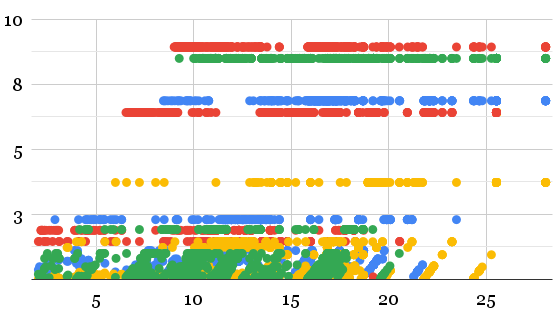
\includegraphics[width=1\linewidth]{figures/node-correlation-ranking.png}
    \caption{Ranking the correlation between attributes in Dataset B}
    \label{fig:attribute-correlation-ranking-dataset-b}
\end{figure}

The subnets field relates the number of attestation subnets that each node advertises.  Nodes by default advertise 2 attestation subnets, but this Dataset B does not include these nodes, leaving only the nodes that advertise 3 or more subnets.  An increase in the level of attestation subnets that a node advertises is presumed to indicate that the node in question has validators attached to it.

The high level of correlation in both the country field and advertised subnets field may indicate that there is a concentration in terms of geographical location of validator nodes.  This corresponds broadly with the observed geographical centralization in network nodes in general for both client and execution nodes \cite{nodewatch2024}.

\subsection{Ranking the level of correlation between attributes in Dataset C}

The same analysis was applied to dataset C, the results of which are displayed in \ref{fig:attribute-correlation-ranking-dataset-c}.  The scatter-plot displays nodes that have more overall correlation between attributes to the right.  As can be observed, the highest level of correlation is found in the top right quadrant of the chart, where there are clear levels of correlation between client, country and the number of validators attached to the node.  This aligns with the results displayed in table \ref{tab:pairwise-comparisons-dataset-c}, that shows similar levels of correlation.

It is worth noting that while including the validator count as a variable in this analysis seems counter-intuitive due to the fact that is a continuous variable, as opposed to categorical like the other attributes, there are broad categories within the data, such as solo stakers for example, and many medium sized stakers, all of whom share similar numbers of validators, making the variable suitable for inclusion.

The correlation between validators and country is based on the number of validators have in common, which does not necessarily indicate a linear relationship, where an increase in the number of validators increases the probability of being in a certain country.  The highest common number of validators is 1, with the mode being .... and median being ....

This may explain the contradictory results in table \ref{tab:pairwise-comparisons-dataset-b}, which shows a relatively low level of correlation between advertised subnets and the country of operation.

\begin{figure}[htbp]
    \centering
    \LARGE \textcolor{bluebullet}\textbullet\ \normalsize Validators % \ % \
    \LARGE \textcolor{redbullet}\textbullet\ \normalsize Client % \ % \
    \LARGE \textcolor{yellowbullet}\textbullet\ \normalsize Country % \ % \
    \LARGE \textcolor{greenbullet}\textbullet\ \normalsize ISP
    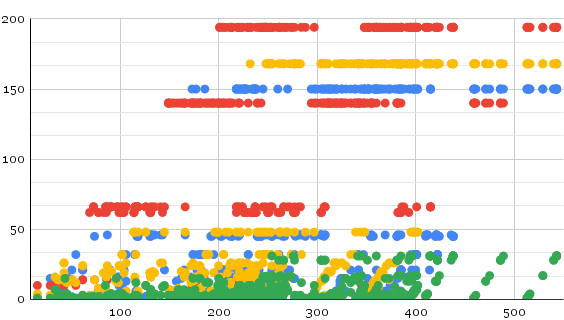
\includegraphics[width=1\linewidth]{figures/chart-3.png}
    \caption{Ranking the correlation between attributes in Dataset C}
    \label{fig:attribute-correlation-ranking-dataset-c}
\end{figure}

\section{Discussion}

Overall the results identified a number of broad observable trends:

Larger node operators tend to propose blocks from more relayers then smaller operators and solo stakers, who tend to propose blocks from only one or a small set of relayers.  This can potentially be explained by solo stakers winning less blocks, but also might be an indication that solo stakers connect to fewer relayers, though without more data it is difficult to disambiguate.

There is a moderate level of correlation between the ISP used and the number of attestation subnets advertised, which may suggest that nodes that have multiple validators attached, usually larger node operators, are often using the same public cloud providers, such AWS or Azure.

The Prysm consensus client has a larger average percentage of use among larger node operators, whereas Nimbus and Lighthouse have less. This observed trend could potentially be attributed to the fact that Lighthouse has been reported to be highly stable and performant, making it a preferred choice in for larger node operators, whereas Nimbus requires less hardware resources, possibly making it more appealing to solo stakers \cite{ranjan2023}.

We observe indications that there is a concentration of geographical location of validator nodes, which corresponds broadly with the observed geographical centralization of all nodes on the network, i.e. validators nodes and non-validator nodes together. However, the discrepancy between the high correlation of geographical location and number of attached validators (see \ref{fig:attribute-correlation-ranking-dataset-c}), with the low level of correlation between geographical location and ISP subnets advertised, (see \ref{fig:relative-level-of-correlation-between-attributes}), suggests that geographical concentration may in fact be driven more by smaller node operators and solo stakers, rather than by larger node operators.  This could be due in part to geographical diversity policies of staking pools such as Lido \cite{vanom2024}.

In summary, it would appear that there is both a slightly lower degree of client diversity, as well as a higher concentration of nodes in public could data centres, that can attributed to larger node operators.  However, larger node operators tend to increase the diversity in mev-boost relays used, and there are indications that they may favor geographical diversity of nodes.

\section{Conclusion}

Observing the percentage breakdown of certain aspects of the node distribution within the network can reveal important insights.  The insights include any unequal distribution of client software used by nodes, or unequal distribution of geographical region of operation.  Both concerns may have implications for the health of the network.  However, by looking at the level of correlation between staking pools and node operators on the network, we can reveal useful clues as to where the drivers of any concentration occurs.  For example, observed trends from our results suggest that larger node operators are potential driving a concentration in certain areas, though to a degree that is not concerning, as indicated by a modified HHI value of 0.

Further to identifying potential drivers of concentration through looking at patterns of correlation, there is also a benefit in developing a standardized index for the measurement of decentralization.  While it can be useful to look at individual aspects of a network, such as geographical distribution of nodes, distribution of nodes by public cloud provider, distribution of client software used etc., it can be a challenge to agree on the overall effect level of decentralization when these various measurements are combined.  This can be all the more challenge when attempting the measure any changes in the overall effective level of decentralization over time.  Similar challenges in traditional economic sectors led to the development of economic indices such as the Gini Index and Herfindahl–Hirschman Index.  For the same reason, it is useful to have a standard index that can be applied to cryptocurrency networks to derive a high-level, comparative measurement.

The modified HHI proposed in this paper can be applied to other areas as well.  In the future the same model can be applied to Layer 2 rollups as they start to decentralize their sequencers.  When this starts to happen, we may have a scenario where some L2s will have a large market share, but will be fully centralized, where other L2s will have a smaller market share and will have fully decentralized sequencers and/or provers.  In this scenario, simply measuring decentralization via observing the relative market share of each L2 is insufficient to capture the effective level of decentralization within the ecosystem.  There may emerge several nuanced factors that should be considered within a decentralized sequencer set, or a shared sequencer network, such as governance parameters, geographic distribution of nodes, or the jurisdiction of headquarters of companies of validator node operators.  It may be the case that some L2 have a rich client diversity within their validator set whereas others do not.  These considerations can be used in conjunction with existing models such as existing methodologies and frameworks \cite{l2beat2024}.

It is worth noting that it is currently quite challenging to collect accurate data on the  correlation between validators and nodes, and node operators.  This is in part by design, as the protocol is designed in such a way as to protocol the identity, including the IP address, of validator nodes.  This provides a level of protection from DDOS attacks, which could have economic consequences if the validator if known to be a proposer and is not able to deliver a block to the network.  However, this also makes it challenging to measure the level of correlation between nodes, which can point to the drivers of concentration in certain areas.

\section*{Acknowledgment}

The authors would like to thank Vitalik Buterin for his time, and insights into developing an index that uses a correlation factor, and would like to thank Elias Sismos at Rated for his advice on using their data.

\printbibliography

\end{document}